\documentclass[10pt, conference]{IEEEtran}
\IEEEoverridecommandlockouts
\usepackage{cite}
\usepackage{amsmath,amssymb,amsfonts}
\usepackage{graphicx}
\usepackage{url}
\usepackage{textcomp}
\usepackage{xcolor}
\usepackage{booktabs}
\usepackage{multirow}
\usepackage{tikz}
\usetikzlibrary{shapes, arrows, positioning, fit, backgrounds, calc}

% figures: July-12 assets in ./figs/, multi-terrain plots in ./figures/
\graphicspath{{figs/}{figures/}{../img/}}

\begin{document}

\title{Nomadic-Node Mobility and Ground-Robot Connectivity Across Terrains:\\
A Protocol-in-the-Loop 5G Emulation Study for Search-and-Rescue}

\author{
\IEEEauthorblockN{Innocent N. Makhubela}
\IEEEauthorblockA{\textit{Dept. of Electrical Engineering} \\
\textit{University of Cape Town} \\
Cape Town, South Africa}
\and
\IEEEauthorblockN{Joyce Mwangama}
\IEEEauthorblockA{\textit{Dept. of Electrical Engineering} \\
\textit{University of Cape Town} \\
Cape Town, South Africa}
\and
\IEEEauthorblockN{Author Three}% TODO: name
\IEEEauthorblockA{\textit{Department TODO} \\
\textit{Institution TODO} \\
City, Country}
\and
\IEEEauthorblockN{Author Four}% TODO: name
\IEEEauthorblockA{\textit{Department TODO} \\
\textit{Institution TODO} \\
City, Country}
\and
\IEEEauthorblockN{Author Five}% TODO: name
\IEEEauthorblockA{\textit{Department TODO} \\
\textit{Institution TODO} \\
City, Country}
\and
\IEEEauthorblockN{Author Six}% TODO: name
\IEEEauthorblockA{\textit{Department TODO} \\
\textit{Institution TODO} \\
City, Country}
}

\maketitle

\begin{abstract}
A UAV-mounted 5G base station---a \emph{nomadic node}---can restore on-demand
connectivity to ground robots performing search-and-rescue (SAR) where terrestrial
infrastructure is absent. A basic operational question is how the robots' links
respond when the drone \emph{moves}, and how that answer changes with the
surrounding terrain, whose obstacles reshape the air-to-ground (A2G) channel. We
answer this empirically with a protocol-in-the-loop emulation that couples a
physics simulator to a real 5G standalone stack: the three-dimensional motion of a
UAV-gNB and two ground-robot user equipments (UEs) continuously drives a
terrain-parameterized A2G path-loss model whose output is injected at runtime into
an OpenAirInterface gNB and UEs, over which genuine TCP, fixed-rate UDP video, and
command-and-control (C2) traffic are measured in both directions across the
emulated air interface. We instantiate five terrains---open field, urban, forest,
hills, and an enterable building---each sharing one obstacle geometry between the
rendered world and the radio channel, and run each as a 6-hour trial split into a
\emph{static}-gNB phase and a \emph{nomadic}-gNB phase while both robots patrol.
The effect of drone mobility on connectivity is strongly terrain-dependent and
changes sign with how pervasively the terrain blocks the link: nomadism rescues a
weak-link robot in line-of-sight (open field, C2 availability $56.5\%\!\to\!88.7\%$),
is neutral under localized building shadowing (urban, ${\sim}96\%$ throughout), and
degrades connectivity as blockage becomes pervasive (hills $-10.6$, forest $-22$
percentage points, with forest video loss exceeding $70\%$). We further show that
maintaining connectivity in non-line-of-sight (NLoS) requires a coverage governor
that reacts to \emph{measured} path loss rather than geometric distance, and that
deep outdoor-to-indoor penetration is effectively uncoverable at this link budget.
We give the complete stack, the geometry-to-signal pipeline, and the emulation
correctness safeguards, and release the testbed and dataset.
\end{abstract}

\begin{IEEEkeywords}
UAV-enabled networks, non-terrestrial networks, nomadic base station, 5G NR,
air-to-ground channel, propagation, search and rescue, protocol-in-the-loop
emulation, OpenAirInterface.
\end{IEEEkeywords}

\section{Introduction}
Search-and-rescue (SAR) operations frequently occur where terrestrial cellular
infrastructure is damaged, congested, or absent: collapsed structures, wildfire
fronts, flood zones, remote wilderness. A UAV carrying a base station---a
\emph{nomadic node}---can restore connectivity on demand, serving ground robots
that stream sensor data and live video to a command post while receiving
navigation waypoints and safety-critical commands in return
\cite{zeng2016wireless, zeng2019accessing, mozaffari2019tutorial}. The concept and
its analytic A2G channel models are well established
\cite{alhourani2014optimal, 3gpp36777}. Because the base station is itself mobile,
a mission planner faces a decision a fixed tower never poses: as the robots spread
through the search area, should the drone \emph{hover} at a vantage point or
\emph{roam} to follow them?

The answer cannot be geometry alone, because the robots operate \emph{in terrain}.
Buildings cast radio shadows; tree canopies attenuate in proportion to the foliage
path length; hills diffract; walls impose outdoor-to-indoor penetration loss. Each
mechanism loads the A2G channel differently, and moving the drone changes the
\emph{propagation path} through that terrain---sometimes clearing an obstacle,
sometimes introducing one. What is needed is \emph{system-level} evidence: how
does a complete 5G protocol stack---with its scheduler, link adaptation, hybrid
ARQ, and radio-link-failure (RLF) machinery---report the connectivity of two
ground UEs as the aerial cell moves, and how does that report differ from one
terrain to the next?

This paper answers that question empirically. We build a protocol-in-the-loop
emulation in which physics-simulated UAV and robot motion continuously modulates a
live 5G standalone stack carrying measured bidirectional traffic, and we
instantiate five terrains that share a single obstacle geometry between the
rendered world and the injected channel. Our contributions are:
\begin{itemize}
  \item \textbf{A mobility- and terrain-coupled emulation architecture}
  (Section~\ref{sec:arch}--\ref{sec:channel}): the full software stack, its
  inter-component communication, the geometry-to-signal pipeline, and a
  terrain-parameterized A2G channel whose NLoS excess is evaluated on the same
  geometry the physics world renders.
  \item \textbf{A controlled static-versus-nomadic study across five terrains}
  (Section~\ref{sec:results}): each a 6-hour trial reporting both UEs' throughput,
  latency, coverage, and outage, establishing that the sign of the mobility effect
  flips with the pervasiveness of terrain blockage.
  \item \textbf{A propagation-aware coverage governor}
  (Section~\ref{sec:control}) that keeps robots connected in NLoS by reacting to
  measured path loss, without which cluttered terrains suffer an unrecoverable RLF
  cascade, together with the emulation correctness safeguards that make the
  measurements honest.
\end{itemize}

\section{Related Work}
Al-Hourani \emph{et al.}~\cite{alhourani2014optimal} derived the widely used
LoS-probability model for low-altitude platforms and showed that an optimal
altitude balances free-space loss against shadowing; our channel core adopts their
formulation. Surveys by Zeng \emph{et al.}~\cite{zeng2016wireless, zeng2019accessing}
and Mozaffari \emph{et al.}~\cite{mozaffari2019tutorial} catalogue UAV-network
design opportunities, and 3GPP studied aerial channel characteristics and
outdoor-to-indoor penetration for cellular UAV support
\cite{3gpp36777, 3gpp38901}. Terrain-specific excess loss has long-standing
empirical models: the Weissberger vegetation model for foliage
\cite{weissberger1982} and knife-edge diffraction for terrain obstruction
\cite{ituP526}. This body of work is predominantly analytic or link-level. We
complement it with protocol-stack-in-the-loop measurement over real bidirectional
traffic, and---in contrast to the common open-field or single-environment
setting---\emph{across five distinct terrains under a common testbed}. On tooling,
OpenAirInterface (OAI) provides an open, 3GPP-compliant RAN with a runtime
channel-model interface \cite{nikaein2014oai}; Open5GS provides the 5G core
\cite{open5gs}; Gazebo provides robotics physics \cite{koenig2004gazebo}. To our
knowledge the specific combination---physics-simulated multi-robot mobility
continuously modulating a live 5G SA stack that carries measured bidirectional
traffic, parameterized across terrains---has not previously been characterized for
SAR.

\section{Why Protocol-in-the-Loop Emulation}
Three methods exist for studying A2G links: closed-form analysis, packet-level
simulation (e.g., ns-3), and protocol-in-the-loop emulation with a real stack.
Analysis and simulation are fast and scalable but abstract away the very
mechanisms whose behaviour we wish to observe---the MAC scheduler's reaction to
changing SINR, HARQ retransmission under fading, modulation-and-coding adaptation,
and the RLF/re-establishment state machine. Because our question is precisely how
these protocol behaviours manifest as user-visible throughput, latency, and outage
as the drone moves through terrain, we run the \emph{actual} 5G software and let
those behaviours emerge, injecting only the physical-layer channel. This trades
scale (one cell, two UEs) for fidelity---an appropriate trade for a study whose
claims are about mechanism and operational rules, not capacity planning.

\section{System Architecture}
\label{sec:arch}
The testbed runs three concurrent control loops on a single host
(Fig.~\ref{fig:arch}); Fig.~\ref{fig:world} shows a rendered instance. The
\emph{channel loop} (2~Hz) reads poses, computes terrain-aware A2G path loss, and
injects it into the live RAN. The \emph{traffic loop} (${\sim}$one cycle per robot
every 15--20~s) exercises and measures each link. The \emph{mobility loop} flies
the UAV and drives the robots. Table~\ref{tab:software} lists the inventory; we
motivate each choice below.

\begin{figure}[t]
\centering
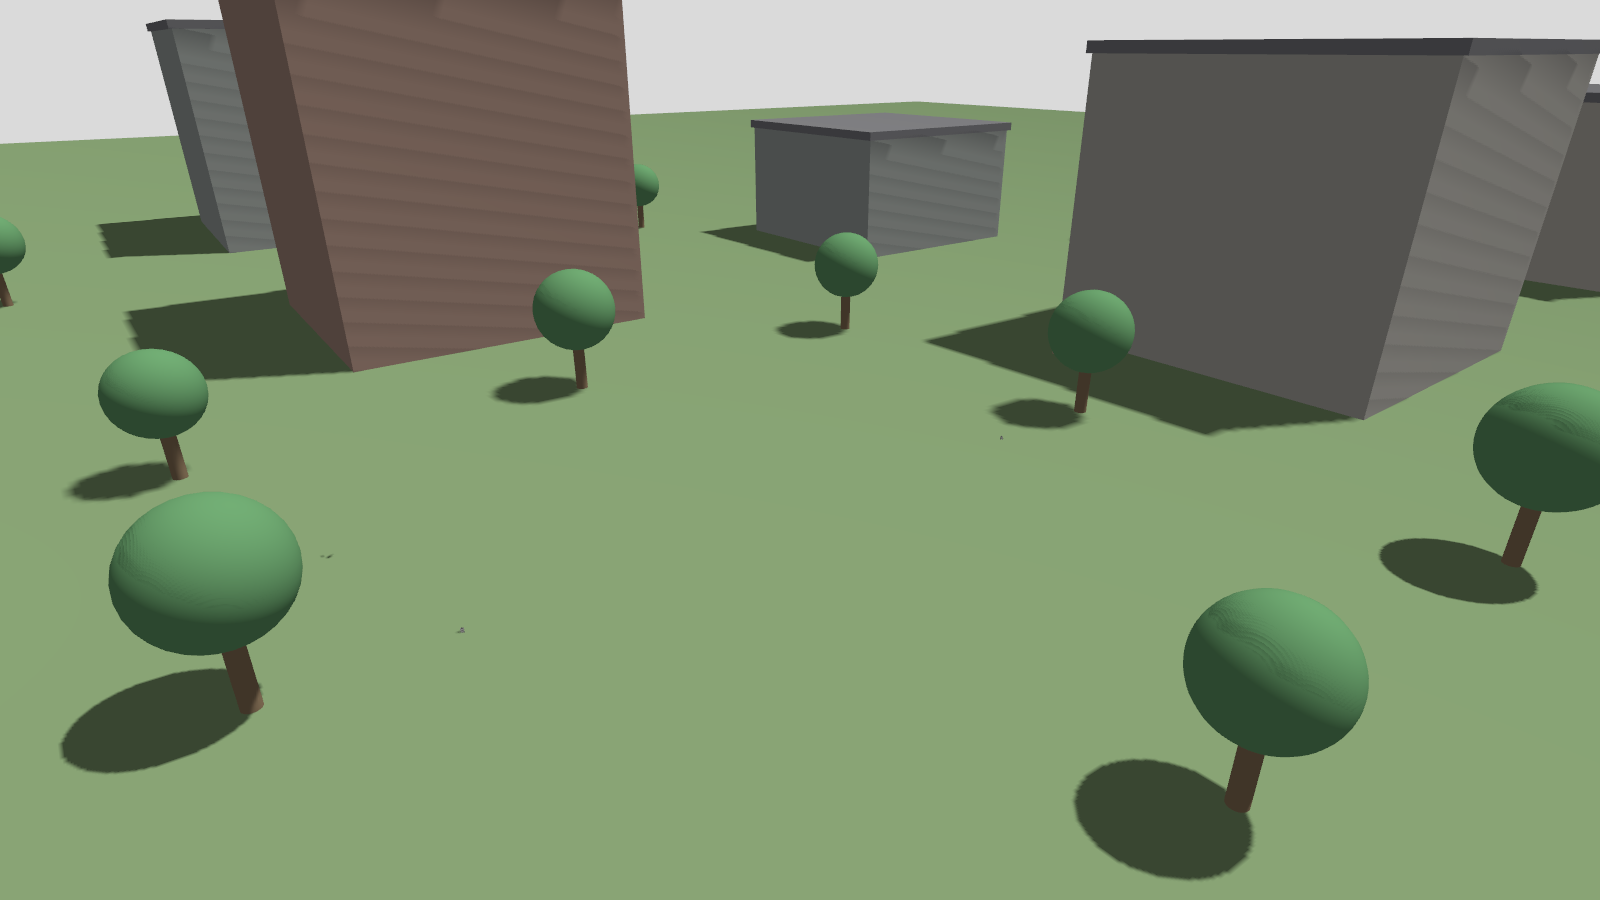
\includegraphics[width=0.94\columnwidth]{gazebo_scene.png}
\caption{A rendered terrain instance (urban). The x500 UAV carries the gNB; two
TurtleBot3 robots are the ground UEs. The same building footprints seen here are
imported by the channel bridge so the radio shadowing matches the visible scene.}
\label{fig:world}
\end{figure}

\begin{table}[t]
\caption{Software stack and roles}
\label{tab:software}
\centering
\footnotesize
\begin{tabular}{@{}lll@{}}
\toprule
\textbf{Component} & \textbf{Version} & \textbf{Role} \\
\midrule
Ubuntu Linux & 22.04 LTS & Host OS (single machine) \\
Gazebo Sim (Harmonic) & 8.x & Physics; publishes 3-D poses \\
gz-transport / gz-msgs & 13 / 10 & Pub/sub bus (Python) \\
PX4 Gazebo model & x500 & UAV/gNB carrier \\
TurtleBot3 (Gazebo) & burger & Two ground-robot UEs \\
OpenAirInterface & 2026.w2x & 5G NR SA RAN + rfsimulator \\
Open5GS & 2.8 & 5G core (AMF/SMF/UPF/\ldots) \\
MongoDB & 6.0 & Subscriber database \\
Python & 3.10 & Bridge, mobility, analysis \\
iproute2 & 5.15 & Per-robot network namespaces \\
iperf3 & 3.16 & TCP/UDP generation \& measurement \\
\bottomrule
\end{tabular}
\end{table}

\begin{figure}[t]
\centering
\begin{tikzpicture}[
  font=\scriptsize, node distance=0.45cm,
  box/.style={rectangle, draw, rounded corners, align=center, inner sep=3pt,
              fill=blue!5, minimum height=0.7cm},
  core/.style={rectangle, draw, rounded corners, align=center, inner sep=3pt,
               fill=green!8, minimum height=0.7cm},
  chip/.style={rectangle, draw, rounded corners, align=center, inner sep=2pt,
               fill=black!4, font=\tiny, minimum height=0.5cm},
  ar/.style={-latex, thick, blue!55!black},
  lbl/.style={font=\tiny\itshape, text=black!60}
]
\node[box, text width=8cm] (gz) {\textbf{PHYSICS + TERRAIN --- Gazebo Harmonic}\\[2pt]
  \begin{tikzpicture}[baseline]
   \node[chip,text width=1.9cm](u){sar\_uav (x500)\\\emph{carries gNB}};
   \node[chip,text width=2.1cm,right=0.25cm of u](a){sar\_ground\_alpha\\UE $\alpha$};
   \node[chip,text width=2.1cm,right=0.25cm of a](b){sar\_ground\_bravo\\UE $\beta$};
  \end{tikzpicture}};
\node[box, text width=8cm, below=0.9cm of gz] (br)
  {\textbf{CHANNEL BRIDGE --- Python}\\[1pt]
   geometry $\rightarrow$ A2G loss $L$ + terrain excess $\Delta_{\mathrm{env}}$
   $\rightarrow$ attenuation $A$};
\node[box, text width=4.6cm, below=0.9cm of br.south west, anchor=north west] (ran)
  {\textbf{5G RAN --- OpenAirInterface}\\[1pt]
   rfsimulator + channelmod\\ n78, 106 PRB, 30 kHz};
\node[core, text width=2.9cm, right=0.35cm of ran] (cn)
  {\textbf{5G CORE --- Open5GS}\\ AMF/SMF/UPF\\ +MongoDB};
\node[box, text width=8cm, below=0.9cm of ran.south west, anchor=north west] (ns)
  {\textbf{PER-ROBOT NETWORK NAMESPACES}\\[1pt]
   robot\_alpha / robot\_bravo --- force DL/UL over the air};
\node[box, text width=8cm, below=0.7cm of ns] (tr)
  {\textbf{TRAFFIC \& MEASUREMENT}\\[1pt]
   iperf3, ping, logger $\rightarrow$ CSV $\rightarrow$ analysis};
\draw[ar] (gz) -- node[lbl,right]{pose/info, gz-transport, $\sim$10 Hz} (br);
\draw[ar] (br.south) -- ++(0,-0.45) -| node[lbl,pos=0.25,right]{telnet channelmod, gain $=-A$, 2 Hz} (ran.north);
\draw[ar,<->] (ran) -- node[lbl,above]{N2/N3} (cn);
\draw[ar] (ran) -- node[lbl,right]{UE TUN} (ns);
\draw[ar] (ns) -- node[lbl,right]{TCP/UDP/ICMP/C2 over the air} (tr);
\end{tikzpicture}
\caption{Testbed architecture. The channel loop (pose $\rightarrow$ bridge
$\rightarrow$ RAN) closes the coupling between physical motion \emph{in terrain}
and radio conditions; user traffic is measured over the emulated air interface
after namespace isolation.}
\label{fig:arch}
\end{figure}

\textbf{Physics and terrain (Gazebo).} Gazebo provides rigid-body motion, a
transport bus for streaming ground-truth poses at ${\sim}10$~Hz, and standard
robot models (PX4 x500 airframe carrying the gNB; TurtleBot3 ground robots as
UEs). Each terrain is a Gazebo world whose obstacle geometry---building footprints,
tree positions, terrain height field, or building walls---is authored once and
\emph{shared} with the channel model, so the radio shadowing is consistent with the
visible scene by construction.

\textbf{5G RAN (OpenAirInterface).} OAI is a real, 3GPP-compliant 5G NR standalone
implementation, so the scheduler, HARQ, link adaptation, and RLF are genuine, not
modelled. Its \texttt{rfsimulator} backend replaces the RF front-end with a
software channel between gNB and UE I/Q streams and exposes a runtime
channel-model control interface (\texttt{channelmod}) through which per-link path
loss can be updated live---exactly the hook the mobility coupling requires.
srsRAN was considered but its channel emulation is less amenable to live per-link
injection; commercial stacks are closed; pure simulators lack the real protocol
implementation that is the point of the study.

\textbf{5G core (Open5GS) and subscribers.} Open5GS supplies a production-grade 5G
core (AMF/SMF/UPF and supporting functions) with a MongoDB subscriber database, so
UE attach and PDU-session establishment are genuine NAS/NGAP/PFCP procedures
rather than shortcuts. Each UE terminates in a host TUN interface.

\textbf{Traffic-path isolation (namespaces).} Linux network namespaces move each
UE's TUN into its own namespace after attach; the modem keeps its open file
descriptor across the move, so the RAN is untouched, but base-to-robot traffic now
genuinely traverses core$\rightarrow$gNB$\rightarrow$radio in both directions
(Section~\ref{sec:pitfalls}). \texttt{iperf3} generates and measures flows;
\texttt{ping} measures latency and delivery; a logger joins each cycle's
measurements with the concurrent geometry into one CSV row.

\section{Geometry and the Terrain-Parameterized A2G Channel}
\label{sec:channel}
The channel is driven entirely by instantaneous geometry. With the UAV at
$(x_u,y_u,h_u)$ and a robot at $(x_r,y_r,h_r)$, the horizontal distance, slant
distance, and elevation angle are
\begin{align}
d_h &= \sqrt{(x_u-x_r)^2 + (y_u-y_r)^2},\\
d_{3D} &= \sqrt{d_h^2 + (h_u-h_r)^2},\\
\theta &= \arctan\!\big[(h_u-h_r)/d_h\big]\ (\mathrm{deg}).
\end{align}
Equations (1)--(3) encode the core insight: two robots at equal map distance $d_h$
can experience very different links, because the radio responds to the slant path
and, decisively, the elevation angle. The free-space loss over the slant path at
carrier frequency $f$ is
\begin{equation}
L_{\mathrm{FSPL}} = 20\log_{10}(d_{3D}) + 20\log_{10}(f) - 147.55.
\end{equation}
Following \cite{alhourani2014optimal}, the LoS probability is a sigmoid in
elevation angle and the base loss adds an angle-dependent excess:
\begin{align}
P_{\mathrm{LoS}}(\theta) &= \frac{1}{1 + a\,\exp[-b(\theta-a)]},\\
L_0 &= L_{\mathrm{FSPL}} + P_{\mathrm{LoS}}\,\eta_{\mathrm{LoS}}
       + (1-P_{\mathrm{LoS}})\,\eta_{\mathrm{NLoS}},
\end{align}
with $a=9.61$, $b=0.16$, $\eta_{\mathrm{LoS}}=1$~dB, $\eta_{\mathrm{NLoS}}=20$~dB.

\textbf{Terrain excess.} The distinguishing element of this study is an additive
terrain term $\Delta_{\mathrm{env}}$ evaluated on the \emph{same} geometry that
Gazebo renders (Table~\ref{tab:terrain}). For \emph{urban}, if the UAV$\to$robot
segment intersects a building footprint the link is hard-NLoS (excess up to
$\eta_{\mathrm{NLoS}}$); otherwise it is clear. For \emph{forest},
$\Delta_{\mathrm{env}}$ grows with the foliage path length through tree canopies
(Weissberger form~\cite{weissberger1982}). For \emph{hills}, it is knife-edge
diffraction over the terrain profile~\cite{ituP526}. For \emph{indoor}, a 3GPP
outdoor-to-indoor term applies whenever the robot is inside the building
footprint---a fixed wall-penetration loss plus a per-metre depth
loss~\cite{3gpp38901}. The total loss is
\begin{equation}
L = L_0 + \Delta_{\mathrm{env}}(\text{UAV},\text{robot},\text{geometry}) + X_\sigma,
\end{equation}
where $X_\sigma$ is correlated log-normal shadow fading (larger variance under
NLoS), decorrelated over distance moved so a stationary robot holds a steady offset.
The bridge references $L$ to $L_{\mathrm{ref}}=L_0(d{=}50\,\mathrm{m},h{=}30\,\mathrm{m})$,
offsets by a per-link baseline $L_{\mathrm{base}}$ (8~dB for $\alpha$'s uplink,
13~dB for $\beta$'s---a 5~dB gap emulating a weaker device class), and clips:
\begin{equation}
A = \mathrm{clip}\big(L_{\mathrm{base}} + (L - L_{\mathrm{ref}}),\, 0,\, 45\big)\ \text{dB}.
\end{equation}
Because OAI's channel field is applied as a linear \emph{gain}
(Section~\ref{sec:pitfalls}), the value written to the RAN is $-A$, scaling each
I/Q sample by $10^{-A/20}$---a true attenuation. Fig.~\ref{fig:parity} shows the
emulated result matches the model to ${\sim}1.2$~dB.

\begin{table}[t]
\caption{The five terrains and their NLoS mechanism}
\label{tab:terrain}
\centering
\footnotesize
\begin{tabular}{@{}lll@{}}
\toprule
\textbf{Terrain} & \textbf{Obstacle} & \textbf{Excess $\Delta_{\mathrm{env}}$} \\
\midrule
Open field & none & graded angle excess only (LoS) \\
Urban & building footprints & hard blockage (segment test) \\
Forest & tree canopies & foliage path length (Weissberger) \\
Hills & terrain height field & knife-edge diffraction \\
Indoor & enterable building & 3GPP O2I: wall + depth loss \\
\bottomrule
\end{tabular}
\end{table}

\begin{figure}[t]
\centering
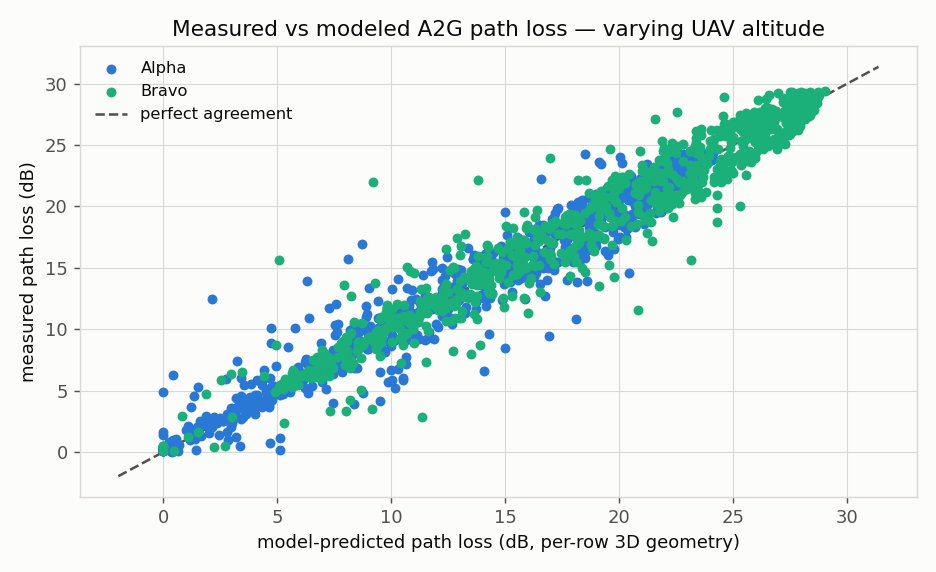
\includegraphics[width=0.82\columnwidth]{parity.png}
\caption{Channel validation: emulated injected path loss vs.\ per-sample model
prediction, on the diagonal (MAE ${\sim}1.2$~dB). The measurements below are a
consequence of the intended physics, not artifacts.}
\label{fig:parity}
\end{figure}

\section{Traffic Model and Metrics}
\label{sec:metrics}
Each measurement cycle exercises a UE with three traffic types mirroring SAR usage.
\textbf{Bulk upload (TCP):} a short \texttt{iperf3} transfer (robot$\rightarrow$base,
slow-start excluded), modelling a sensor dump; goodput reflects reliable-transport
capacity. \textbf{Video (UDP):} a fixed 8~Mbit/s uplink stream modelling a live
camera; delivered rate, loss, and jitter reflect stream quality. \textbf{Command
\& Control (C2):} five 64-byte ICMP pings \emph{base$\rightarrow$robot}, emulating
the downlink control channel (navigation waypoints, emergency-stop). C2 is the
safety channel: its RTT and loss measure \emph{controllability}---the ability to
steer or halt a robot---not bandwidth. We also record UE-reported RSRP and SINR,
and define \emph{coverage/C2 availability} (fraction of samples with less than
$100\%$ C2 loss), \emph{outage probability} (fraction in total loss), and
inter-robot Jain fairness. Because both robots are logged every cycle, all metrics
are reported per UE ($\alpha$ = stronger budget, $\beta$ = weaker).

\section{Mobility and Propagation-Aware Coverage Governance}
\label{sec:control}
Robots drive by differential-drive velocity commands at 1~m/s along randomized
continuous headings---genuine kinematics, not teleportation. In each trial the UAV
first \emph{hovers} statically, then performs a continuous three-dimensional random
walk over a bounded box (Section~\ref{sec:setup}). To keep robots from being
stranded as coverage moves, a governor confines each robot. A naive governor uses a
geometric \emph{safe radius} from the open-field model,
\begin{equation}
\label{eq:rsafe}
R_{\mathrm{safe}}(h)=\max\{ d_h : L_{\mathrm{base},\beta}+[L_0(d_h,h)-L_{\mathrm{ref}}]\le A_{\mathrm{safe}}\},
\end{equation}
with $A_{\mathrm{safe}}{=}30$~dB (${\approx}5$~dB below the RLF cliff), evaluating
to $101/131/163$~m at $h{=}20/40/60$~m. \textbf{This fails in NLoS:} a robot can
sit well inside $R_{\mathrm{safe}}$ yet be blocked by a building or canopy (path
loss near the cliff), because the distance rule is blind to obstacles. Worse, once
such a UE loses the link it declares RLF, and because a UE cannot complete cell
(re)synchronization while buried in deep NLoS, restarting it \emph{fails to
re-attach}---the recovery loops indefinitely and the robot stays dark. We therefore
make the governor react to \emph{measured} path loss: when a UE's loss is elevated
it is steered toward the gNB ground track (raising the elevation angle and reducing
NLoS depth), and if loss stays near the cliff the robot is relocated to a small
radius from the gNB \emph{before} it dies. For the indoor mission, where the robot
must occupy the building, it instead retreats toward the door (reducing penetration
depth) and re-enters on recovery. This prevention-first design converts an
unrecoverable cascade into rare, short outages (Section~\ref{sec:results}).

\subsection{Emulation correctness safeguards}
\label{sec:pitfalls}
Building an honest single-host testbed surfaced three failure modes producing
\emph{plausible but wrong} data; all reported results were collected only after all
three were fixed. \emph{(i)~The channel field is a gain, not a loss.} OAI's
\texttt{channelmod} applies \texttt{path\_loss\_dB} as a linear gain
($10^{x/20}$)---positive values \emph{amplify}---so positive ``loss'' produced a
link that degraded only via sample clipping and UE RSRP that \emph{rose} with
distance; we keep $A$ positive and negate once at injection~(9).
\emph{(ii)~Single-host traffic bypasses the radio.} With host-local UE IPs,
base-to-robot traffic went over loopback (a ``downlink'' test read Gbit/s while the
gNB scheduled 0.15~Mbit/s); moving each TUN into a per-robot namespace forces the
air path. \emph{(iii)~A single-client control port drops writes.} OAI's telnet
accepts one client per port; a second socket to the gNB port sat unaccepted in the
backlog, silently discarding one UE's uplink modulation. A shared connection per
port with a start-up read-back refuses to run unless every baseline verifies.

\section{Experimental Setup}
\label{sec:setup}
Each terrain runs a single 6-hour trial in two phases: \emph{phase~1} (0--3~h) with
the gNB hovering statically, and \emph{phase~2} (3--6~h) with the gNB performing a
continuous 3-D random walk over a bounded box (never dwelling). Both robots
free-patrol throughout, so the only variable between phases is gNB mobility. The
gNB uses band~n78 (3.32~GHz, 40~MHz, 30~kHz SCS, 106~PRB) on Open5GS. A single
physical stack must serve only one trial---two concurrent trials share the same
robots and gNB and corrupt each other---so trials are serialized under an exclusive
lock. Reported worlds are clean 6-hour trials with 733, 721, 482, and 974 samples
for open field, urban, forest, and hills; the indoor trial is reported separately
as a coverage limit. Exploratory runs collected while the safeguards of
Section~\ref{sec:pitfalls} were latent are excluded from every number.

\section{Results}
\label{sec:results}

\subsection{Propagation and coverage across terrains}
Fig.~\ref{fig:ploss} bins measured path loss against gNB--robot slant distance per
terrain---the physical basis of everything that follows: open field and hills sit low
(shallow, LoS-dominated); forest climbs steeply because a longer slant path cuts
through more canopy; urban is intermediate with building-driven jumps.
Fig.~\ref{fig:covmap} makes the same physics spatial---the link attenuation over the
search area for a static drone (left), and the fraction of time each point is covered
as the drone roams (right). The terrain signature is unmistakable: open field is a
clean radial field, urban is fractured by building shadows, forest disintegrates into
thin coverage fingers, and hills form an irregular covered island. Terrain does not
merely shift coverage---it changes its \emph{shape}, so moving the drone has a
terrain-specific effect.

\begin{figure}[t]
\centering
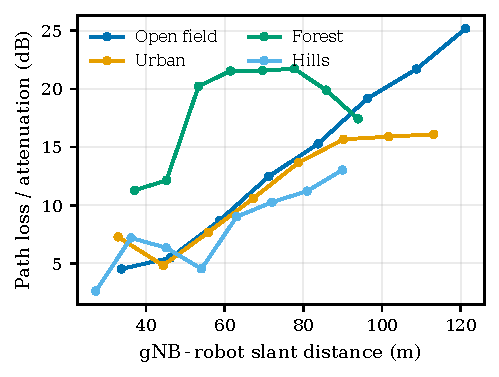
\includegraphics[width=\columnwidth]{fig_ploss_dist.pdf}
\caption{Measured path loss vs.\ gNB--robot slant distance (binned means) per
terrain. Forest rises steeply with distance; open field and hills stay low; urban is
intermediate.}
\label{fig:ploss}
\end{figure}

\begin{figure}[t]
\centering
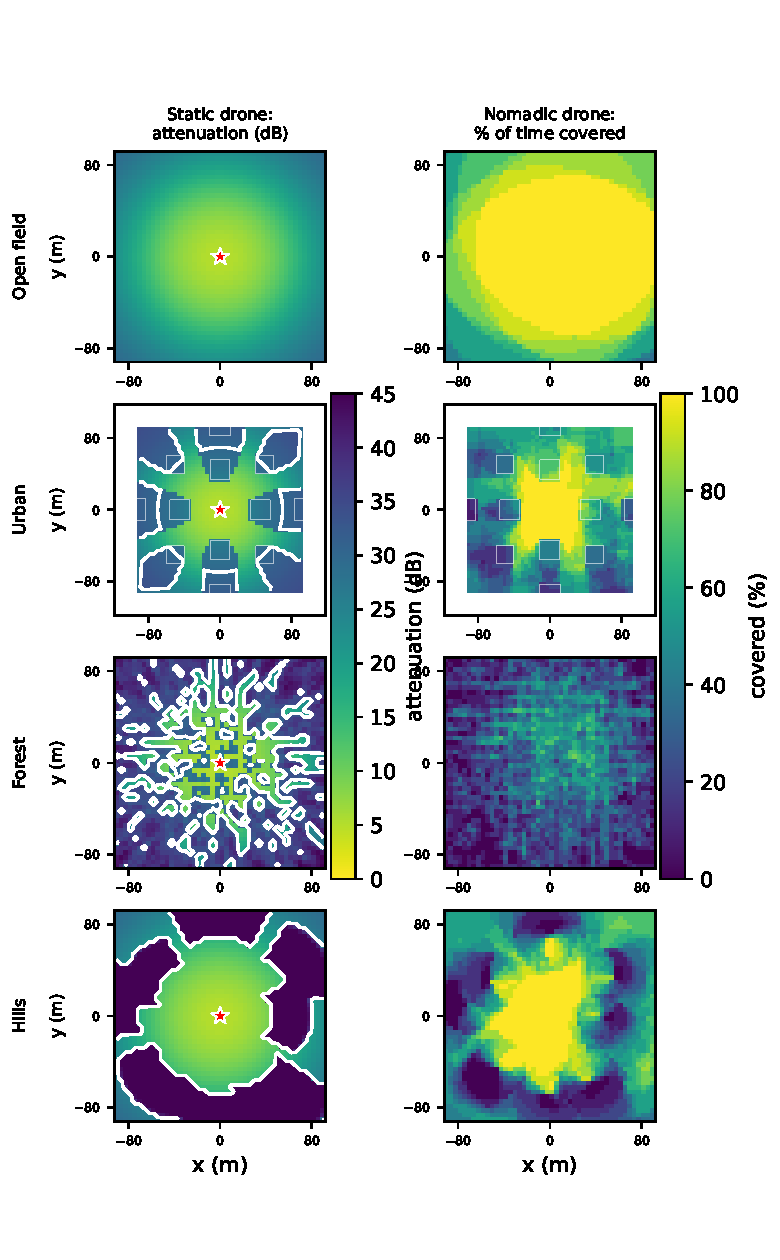
\includegraphics[width=0.9\columnwidth]{fig_coverage_map.pdf}
\caption{Coverage field over the search area (weaker UE), per terrain. Left: link
attenuation for a \emph{static} drone at the origin (red star; white contour = usable
edge). Right: fraction of time each point is covered as a \emph{nomadic} drone roams.
Urban is fractured by building shadows; forest never coheres; open field's field is
radial and spreads as the drone moves.}
\label{fig:covmap}
\end{figure}

\subsection{Watching the drone move}
Fig.~\ref{fig:tsc2} shows the raw phenomenon: both UEs' C2 connectivity over the full
6-hour mission, per terrain, with the static$\to$nomadic transition marked at 3~h
(shaded = nomadic). The effect is legible directly. In \emph{open field}, the weak
UE~$\beta$ repeatedly drops while the gNB is static, then \emph{steadies} once it
roams. In \emph{urban} both UEs stay flat across the transition. In \emph{forest},
both are healthy while static, then connectivity \emph{collapses} the moment the gNB
begins roaming. \emph{Hills} is a milder version. The bars below quantify it.

\begin{figure}[t]
\centering
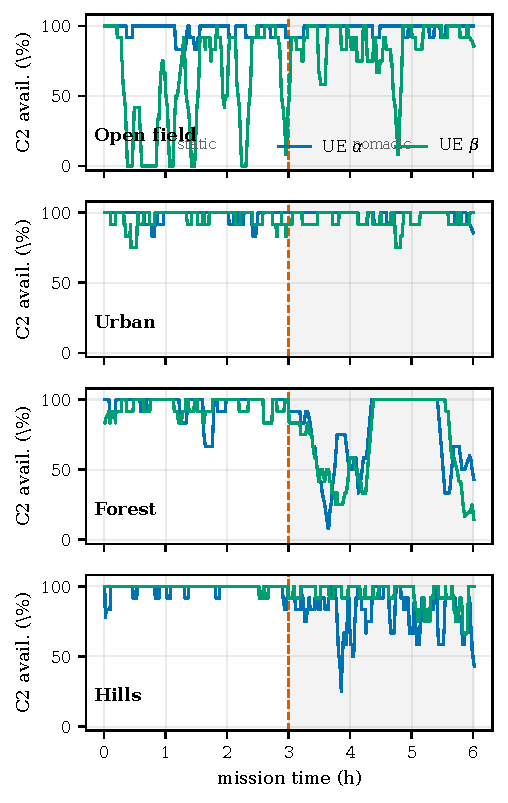
\includegraphics[width=0.86\columnwidth]{fig_ts_c2.pdf}
\caption{C2 connectivity over the 6-hour mission, per terrain, both UEs (rolling
availability); dashed line = static$\to$nomadic transition (3~h), shaded = nomadic.
UE~$\beta$ steadies under nomadism in open field; forest collapses when the drone
starts moving.}
\label{fig:tsc2}
\end{figure}

\subsection{Moving the drone: the effect flips with terrain}
Fig.~\ref{fig:c2} and Table~\ref{tab:main} give the central result:
\textbf{the effect of drone mobility on connectivity is terrain-dependent and changes
sign with the pervasiveness of blockage.} In \emph{open field} (line-of-sight)
mobility \emph{helps} the weak-link robot: $\beta$'s C2 availability rises from
$56.5\%$ (static) to $88.7\%$ (nomadic), a $+32$~pp gain, as the wandering gNB
periodically drifts closer and rescues a robot stranded near the coverage edge (its
mean distance falls from $91$ to $75$~m), while $\alpha$ stays near $98\%$. In
\emph{urban} mobility is \emph{neutral} (${\sim}96$--$98\%$): localized buildings
leave LoS pockets the governor keeps robots in. In \emph{hills} and \emph{forest}
mobility \emph{hurts}, scaling with how pervasive the blockage is---$-10.6$~pp for
knife-edge terrain and $-22$~pp for everywhere-present foliage, which collapses both
UEs to ${\sim}73$--$75\%$.

\begin{figure}[t]
\centering
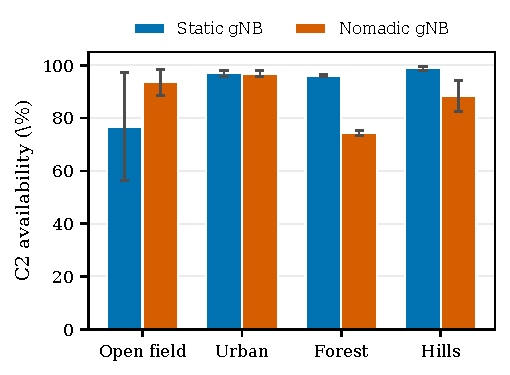
\includegraphics[width=\columnwidth]{fig_c2_avail.pdf}
\caption{C2 availability by terrain and gNB phase (bar = robot mean; whiskers span
the two UEs). Nomadism helps in open field, is neutral in urban, and hurts in hills
and forest.}
\label{fig:c2}
\end{figure}

\begin{table}[t]
\centering
\caption{C2 availability and mean link metrics by terrain and gNB phase
(robot-averaged). $\Delta$ is nomadic$-$static C2 (pp).}
\label{tab:main}
\footnotesize
\begin{tabular}{@{}llrrrr@{}}
\toprule
Terrain & Phase & C2 (\%) & PLoss & SINR & TCP \\
        &       &         & (dB)  & (dB) & (Mb/s) \\
\midrule
\multirow{3}{*}{Open field}
 & Static  & 76.8 & 16.5 & 35.1 & 9.7  \\
 & Nomadic & 93.5 & 14.2 & 38.8 & 13.1 \\
 & \multicolumn{1}{r}{$\Delta$} & \textbf{+16.7} & & & \\
\midrule
\multirow{3}{*}{Urban}
 & Static  & 97.0 & 8.8  & 43.8 & 17.6 \\
 & Nomadic & 96.9 & 10.4 & 42.6 & 16.1 \\
 & \multicolumn{1}{r}{$\Delta$} & \textbf{$-$0.1} & & & \\
\midrule
\multirow{3}{*}{Hills}
 & Static  & 98.9 & 3.9  & 45.7 & 21.6 \\
 & Nomadic & 88.3 & 9.3  & 44.2 & 19.4 \\
 & \multicolumn{1}{r}{$\Delta$} & \textbf{$-$10.6} & & & \\
\midrule
\multirow{3}{*}{Forest}
 & Static  & 96.2 & 10.8 & 40.9 & 15.1 \\
 & Nomadic & 74.2 & 21.7 & 32.5 & 3.2  \\
 & \multicolumn{1}{r}{$\Delta$} & \textbf{$-$22.0} & & & \\
\bottomrule
\end{tabular}
\end{table}

\subsection{What it costs the mission: streaming and control}
Connectivity translates directly into mission capability (Fig.~\ref{fig:video}). The
8~Mbit/s video feed---the operator's eyes---arrives nearly intact in open field,
urban, and hills, but in forest a nomadic drone drives it to $1.9$~Mbit/s with over
$70\%$ loss: the operator goes blind exactly when the drone moves. Command latency,
by contrast, holds near $37$~ms median \emph{whenever the link is up}, in every
terrain and phase---so controllability fails as an \emph{availability} problem (the
command channel is present or absent), not a latency creep.

\begin{figure}[t]
\centering
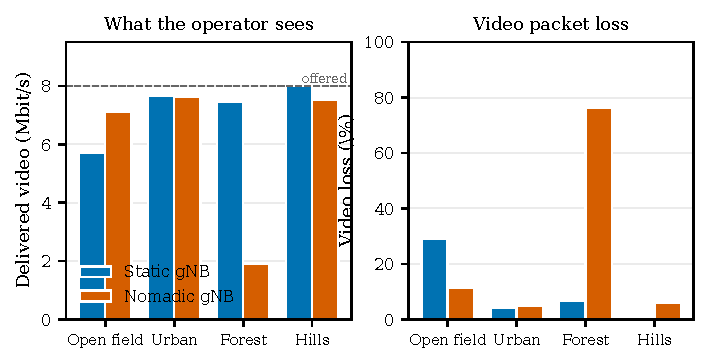
\includegraphics[width=\columnwidth]{fig_video.pdf}
\caption{Delivered video rate and loss, static vs.\ nomadic gNB per terrain. Forest
video collapses to $1.9$~Mbit/s ($>70\%$ loss) under a nomadic drone; open-field
nomadism instead \emph{helps} the weak UE.}
\label{fig:video}
\end{figure}

\subsection{Throughput and coverage as the UE moves}
Fig.~\ref{fig:tputdist} plots TCP goodput against UE--gNB distance, static vs.\
nomadic, per terrain. In open field the static curve falls off a coverage cliff with
range while the nomadic drone flattens it by following the robot; in forest both
curves sit low and nomadism cannot lift them. This is the mobility trade in one view:
moving the drone buys range where the path is clear and buys nothing where it is
blocked.

\begin{figure}[t]
\centering
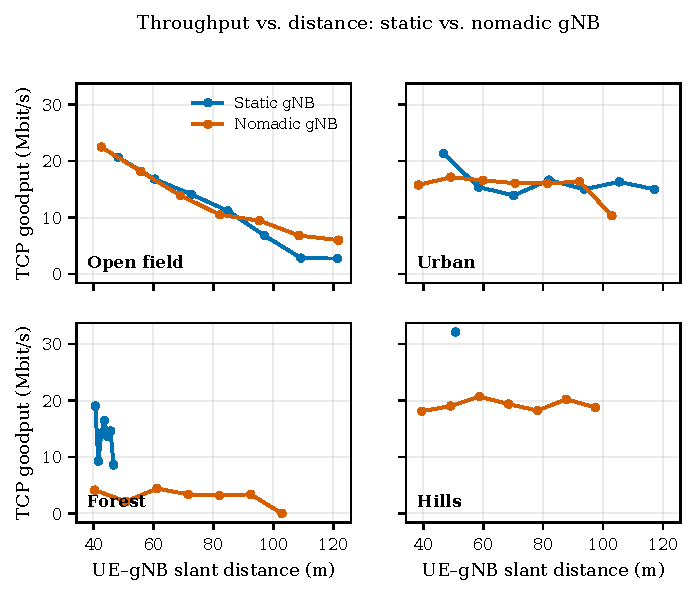
\includegraphics[width=\columnwidth]{fig_tput_distance.pdf}
\caption{TCP goodput vs.\ UE--gNB distance, static vs.\ nomadic gNB, per terrain.
Nomadism flattens the open-field cliff (the drone follows the robot) but cannot lift
the blocked forest link.}
\label{fig:tputdist}
\end{figure}

\subsection{The real stack adapts}
Because we run a genuine RAN, link adaptation is observed, not modelled
(Fig.~\ref{fig:linkadapt}). As the forest-nomadic channel degrades, the scheduler
backs uplink spectral efficiency down ($4.2\!\to\!2.7$~bits/sym) while HARQ holds
block error near target ($<0.04\%$)---the protocol trading rate for reliability,
which a link-level abstraction would miss. This is the payoff of protocol-in-the-loop
emulation.

\begin{figure}[t]
\centering
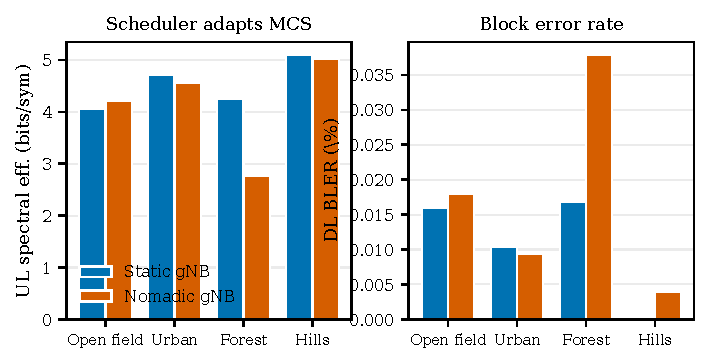
\includegraphics[width=\columnwidth]{fig_linkadapt.pdf}
\caption{Uplink spectral efficiency and downlink BLER, static vs.\ nomadic per
terrain. In forest-nomadic the scheduler drops MCS while HARQ keeps BLER bounded---the
real stack adapting.}
\label{fig:linkadapt}
\end{figure}

\subsection{Device budget and the weakest radio}
Consistent with the open-field baseline, the two UEs differ only by 5~dB of
baseline budget yet experience qualitatively different networks: $\alpha$ is
distance-limited while $\beta$ is budget-limited, reaching the cliff sooner and
defining the team's usable region. High Jain fairness ($J{\approx}0.97$) confirms
the disparity is device budget, not scheduler bias---so the remedy is coverage
margin, and the governor and drone placement must be sized for the \emph{weakest}
radio, in every terrain.

\subsection{Keeping robots connected in NLoS}
Fig.~\ref{fig:events} counts link-recovery events per 6-hour trial. With the
propagation-aware governor, the RLF cascade is eliminated in urban and hills (zero
failed re-attaches) and contained in forest, where the governor intervenes $574$
times---roughly once every $37$~s---to keep robots out of foliage dead zones. The
cost of prevention is a more gNB-centred robot distribution: the governor keeps NLoS
robots closer to the gNB than free roaming would (the concentrated nomadic coverage
of Fig.~\ref{fig:covmap}). This is the price of any valid measurement in NLoS;
without it the cluttered terrains do not merely degrade, they fail to produce data.

\begin{figure}[t]
\centering
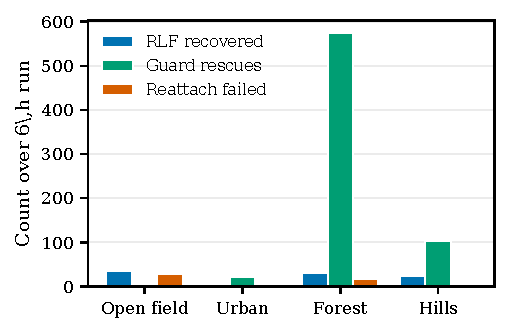
\includegraphics[width=\columnwidth]{fig_events.pdf}
\caption{Link-recovery events per 6-hour trial. Forest requires by far the most
governor interventions; urban and hills incur zero failed re-attaches.}
\label{fig:events}
\end{figure}

\subsection{Indoor: a coverage limit}
The outdoor-to-indoor terrain is qualitatively different (Fig.~\ref{fig:indoor}).
The fixed wall-penetration term plus the link baseline places the \emph{entire}
building interior near the RLF cliff---depth barely matters---so shadow spikes trip
RLF repeatedly, and each ${\sim}2$-minute re-attach dominates the timeline. Lowering
the gNB to hover directly overhead (cutting ${\sim}7$~dB of A2G loss) and adding the
retreat-to-door recovery removes the cascade and keeps robots alive, but C2
availability remains only $12$--$18\%$. We read this as a genuine finding: a ground
robot cannot hold connectivity deep inside a building at this link budget, and
\emph{leaving the building is the only recovery}.

\begin{figure}[t]
\centering
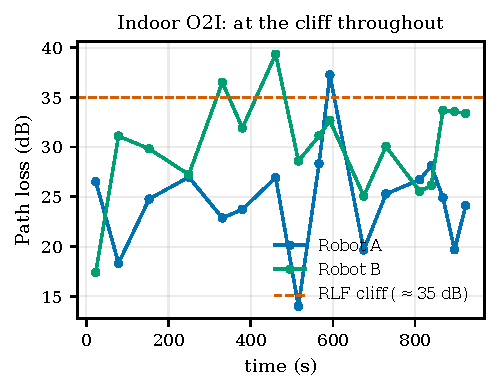
\includegraphics[width=\columnwidth]{fig_indoor.pdf}
\caption{Indoor O2I path loss over time (low-hovering gNB). Both robots sit at the
RLF cliff throughout; the interior offers no reliably covered pocket.}
\label{fig:indoor}
\end{figure}

\section{Discussion}
The unifying explanation is that moving the drone changes the \emph{propagation
path}, and whether that helps depends on how blockage is distributed. In LoS a
moving gNB is pure geometric benefit---it can shorten links and rescue edge
robots---so nomadism helps the weak robot most. Where blockage is \emph{localized}
(urban buildings), a governor can keep robots in LoS pockets and mobility washes
out. Where blockage is \emph{pervasive} (forest canopy) there is no pocket to hold:
any repositioning that lengthens the ground path lengthens the foliage path, so
mobility is strictly harmful, and the damage scales with blockage density
(hills~$<$~forest). Two operating rules follow for SAR: \emph{hover} a nomadic node
when the environment is cluttered and pervasive, and \emph{roam} it only when links
are LoS-dominated or robots risk stranding at the coverage edge; and size coverage
for the weakest radio in the team.

\section{Limitations}
The RAN runs over \texttt{rfsimulator}, so absolute link budgets depend on model
constants and the configured noise floor; we therefore emphasize \emph{relative}
static-vs-nomadic effects within a fixed calibration rather than absolute edges.
The coverage governor is necessary to obtain data in NLoS but alters robot
trajectories (more gNB-centred), so the reported effects are conditional on
prevention-based coverage keeping; free-roaming robots would simply lose the link.
We study one cell and two UEs; multi-cell handover and many-robot contention are
future work. Under outage the per-sample probes time out, so heavily degraded
phases yield fewer samples (e.g., forest phase~2), though fine-grained path loss is
logged continuously by the bridge. The indoor result reflects one building geometry
and link budget. Subject to these, the \emph{direction} of the findings follows
from geometry, link budget, and protocol-state mechanisms that carry to physical
LoS/NLoS deployments.

\section{Conclusion and Future Work}
\label{sec:conclusion}
We presented a mobility- and terrain-coupled 5G emulation testbed for UAV-mounted
nomadic nodes serving ground robots, and used it to measure how two ground UEs
report their connectivity as the drone moves, across five terrains. The effect of
gNB mobility on connectivity is terrain-dependent and changes sign with the
pervasiveness of blockage: helpful in line-of-sight (open field, $+32$~pp for the
weak robot), neutral under localized urban shadowing, and increasingly harmful
under diffraction and foliage (hills $-10.6$, forest $-22$~pp), while deep
outdoor-to-indoor penetration is effectively uncoverable. We further showed that
maintaining connectivity in NLoS requires a governor that reacts to measured path
loss rather than geometric distance, and we documented the emulation safeguards
that make single-host measurement honest. Future work relaxes the single-cell
assumption toward multi-node handover, adds a coverage-edge recovery-time study,
and pursues SDR hardware validation.

\section*{Acknowledgment}
\emph{[Anonymized for double-blind review.]}

\begin{thebibliography}{00}
\bibitem{zeng2016wireless} Y. Zeng, R. Zhang, and T. J. Lim, ``Wireless
communications with unmanned aerial vehicles: Opportunities and challenges,''
\textit{IEEE Commun. Mag.}, vol.~54, no.~5, pp.~36--42, 2016.
\bibitem{zeng2019accessing} Y. Zeng, Q. Wu, and R. Zhang, ``Accessing from the
sky: A tutorial on UAV communications for 5G and beyond,'' \textit{Proc. IEEE},
vol.~107, no.~12, pp.~2327--2375, 2019.
\bibitem{mozaffari2019tutorial} M. Mozaffari, W. Saad, M. Bennis, Y.-H. Nam, and
M. Debbah, ``A tutorial on UAVs for wireless networks: Applications, challenges,
and open problems,'' \textit{IEEE Commun. Surveys Tuts.}, vol.~21, no.~3,
pp.~2334--2360, 2019.
\bibitem{alhourani2014optimal} A. Al-Hourani, S. Kandeepan, and S. Lardner,
``Optimal LAP altitude for maximum coverage,'' \textit{IEEE Wireless Commun.
Lett.}, vol.~3, no.~6, pp.~569--572, 2014.
\bibitem{3gpp36777} 3GPP, ``Study on enhanced LTE support for aerial vehicles,''
TR~36.777, 2017.
\bibitem{3gpp38901} 3GPP, ``Study on channel model for frequencies from 0.5 to
100 GHz,'' TR~38.901, 2020.
\bibitem{weissberger1982} M. A. Weissberger, ``An initial critical summary of
models for predicting the attenuation of radio waves by trees,'' ECAC-TR-81-101,
1982.
\bibitem{ituP526} ITU-R, ``Propagation by diffraction,'' Recommendation P.526.
\bibitem{nikaein2014oai} N. Nikaein \textit{et al.}, ``OpenAirInterface: A flexible
platform for 5G research,'' \textit{ACM SIGCOMM Comput. Commun. Rev.}, vol.~44,
no.~5, pp.~33--38, 2014.
\bibitem{open5gs} Open5GS, ``Open source implementation of the 5G core network,''
\url{https://open5gs.org}, accessed 2026.
\bibitem{koenig2004gazebo} N. Koenig and A. Howard, ``Design and use paradigms for
Gazebo, an open-source multi-robot simulator,'' in \textit{Proc. IEEE/RSJ IROS},
2004, pp.~2149--2154.
\end{thebibliography}

\end{document}
